\chapter{Fundamentals}
\label{chap:fundamentals}

In this chapter we give an explanation about the technologies and concepts this diploma thesis relies on. We start describing the fundamental concepts and introduce the components and prototypes that form the basis of our work.

\section{Cloud Computing}
\label{sec:cloudcomputing}

In the last decades our world has become more and more interconnected. This interconnection added to the increase of the available bandwidth and the change in business models have forced IT Systems to fulfill its demands, leading to its reorganization into a public utility which offers public services, like water, electricity, etc. The \ac{NIST} defines Cloud computing as "a model for enabling ubiquitous, convenient, on-demand network access to a shared pool of configurable computing resources (e.g., networks, servers, storage, applications, and services) that can be rapidly provisioned and released with minimal management effort or service provider interaction"  \cite{NIST2011}. The Cloud computing model is composed of five characteristics:
	\begin{enumerate}
		\item On-demand self-service: a Cloud user consumes the Cloud provider's computing capabilities automatically without the need of human interaction. 
		\item Broad network access: computing capabilities are available via the network and can be accessed using standard mechanisms.
		\item Resource pooling: computing capabilities in the Cloud provider side are virtualized to serve multiple consumers simultaneously using a multi-tenant model. The Cloud consumer generally has no sense of the provided resources.
		\item Rapid Elasticity: computing and storage resources can be dynamically (and in some cases automatically) provisioned and released to respond to the actual consumers' demand.
		\item Measured Service: resources' usage is monitored and measured in a transparent way to the Cloud consumer and provider for control and optimization purposes.
	\end{enumerate}

The control that the Cloud consumer has over the computer resources in a Cloud provider infrastructure is defined in three service models: \term{\ac{SaaS}}, \term{Platform-as-a-Service (\ac{PaaS})} and \term{\ac{IaaS}}. \term{\ac{SaaS}} provides to the Cloud consumer access and usage of Cloud provider's applications running on a Cloud infrastructure. The consumer has no control over the underlying infrastructure where the application he uses is deployed. The customer can only control individual application's configurations during his usage of it. \term{\ac{PaaS}} provides the customer with the needed capabilities to deploy applications which's programming language, required libraries, services and tools are supported by the provider. The consumer has no control over the underlying infrastructure where he deploys the application. \term{\ac{IaaS}} is the model which gives most control to the consumer. Thus, the consumer is able to deploy and run arbitrary software and has the control over operating systems, storage and deployed applications, but has no management or control on the underlaying Cloud infrastructure. 

Although the three service models described above provide both data computation and storage capabilities for the consumer, they do not provide to the customer the possibility to directly and uniquely purchase access of storage services. In this diploma thesis we concentrate in two concrete models: \term{\ac{DBaaS}} and \term{\ac{STaaS}}. Cloud storage providers target a selected number of consumers, who process their data on-premise, but do not  want to cover the expenses of a local database system, or a backup system, among others. The Cloud storage model alleviates the need in organizations to invest in database hardware and software, to deal with software upgrades, and to maintain a professional team for its support and maintenance \cite{dbaasIyer}.  \ac{DBaaS} and \ac{STaaS} can be considered quite similar, except for one of their main distinction characteristics: their access interface. The former is the most robust data solution offered as a service, as it offers a full-blown database functionality. It can be accessed via the most common database protocols, such us MySQL, Oracle, etc, or by REST interfaces supporting \ac{SQL}. Examples of this model are Amazon RDS \cite{amazonrds} and Oracle Cloud \cite{oraclecloud}. On the other hand, the latter provides REST, \ac{SOAP} over \ac{HTTP}, or Web-based interfaces in order to perform the operations over the stored data \cite{cloudstorageWU}. Examples of this model are Amazon Dynamo \cite{amazondynamodb} , Google App Engine Datastore \cite{googleappdatastore}, and Dropbox \cite{dropbox}.

\ac{NIST} defines four deployment models in Cloud computing. A private Cloud consists in a Cloud infrastructure which is provisioned exclusively for one organization and used by the members conforming the organization. It is comparable to processing facilities that are enhanced with the Cloud computing characteristics. A community Cloud is a Cloud infrastructure where its use is limited to organizations which share the same requirements. A public Cloud infrastructure can be accessed and used by the public. It is usually offered by Cloud service providers that sell Cloud services made for general public or enterprises. Some of the Cloud consumers may process and store information which requires more control over the infrastructure in which is located, or consume public Cloud computing resources during peak loads in their private Cloud infrastructure. The hybrid Cloud model combines two or more deployment models described above and the combination remains as a unique entity.  

Cloud computing and \ac{SOA} are related styles at an architectural, solution and service level, according to IBM \cite{IBM2011}. Cloud providers expose their Cloud infrastructure as services as part of a \ac{SOA} solutions and the communication between Clouds in the Hybrid Cloud model described above can be compared to a SOA communication solution between enterprises. Cloud services are services that can be accessed by the Cloud consumers through the network. Therefore, we can deduce that the SOA model can be applied in the Cloud computing approach. As the \ac{ESB} is the central piece of \ac{SOA}, the need of the \ac{ESB} in a Cloud computing infrastructure as an integration middleware for the Cloud services is essential. 
\section{Service-Oriented Architecture}
\label{sec:soa}  

Weerawarana et al. define SOA as an specific architectural style that is concerned with loose coupling and dynamic binding between services \cite{Weera2005}.

In the last years communication between external components whose functionalities are exposed as services has been a hard task when there was not previous agreement on message protocols, data types and encoding, and used middleware technology. Due to the economic and technological growth needed, enterprises had to adapt the \ac{SOA} paradigm in their existing IT Infrastructure. \ac{SOA} provides the needed flexibility by building an architectural style with the following benefits: loose coupling, interoperability, efficiency, and standardization. The W3C group defines SOA as a form of distributed system architecture that is typically characterized by the following properties \cite{w3csoa}:
	\begin{itemize}
		\item Logical view: the service's functionality is exposed, but not its internal logic.
		\item Message orientation: the internal structure of an agent is abstracted.
		\item Description orientation: a service is described by machine-processable meta data.
		\item Granularity: services tend to use a small number of operations with relatively large and complex messages.
		\item Network orientation: Services tend to be oriented toward use over a network.
		\item Platform neutral: Messages are sent in a platform-neutral, standardized format delivered through the interfaces.
	\end{itemize}

\ac{SOA} defines three main roles: requester, provider and broker and the four main operations: publish, find, bind, and invoke. The service provider provides access to services, creates a description of a service and publishes it to the service broker. The service requestor discovers a service by searching through the service descriptions located in the service broker. When the service which best fits to his needs is found, the discovering facility provides the concrete service endpoint and the consumer is responsible for binding to it.  With this information, the requestor can then bind to the concrete service and finally execute a business activity \cite{Weera2005}. The service broker provides support for service registration and binding. 

The main component in a \ac{SOA} is the \ac{ESB}. The functionalities provided by a service bus can simplify the process (publication, discovery, binding, and invocation) and make it more transparent to provide an ease-to-use experience for a Web service based implementation of \ac{SOA} \cite{Weera2005}. Chappel defines its function as an intermediate connection provisioning of service providers with service consumers and thereby ensure decoupling of theses \cite{Chapp2004}. 

\subsection{Enterprise Service Bus}

The flow of data and information is a key for driving business decisions in IT organizations \cite{Chapp2004}. Furthermore, the interaction between loosely coupled components within an organization or with third party organizations requires distributed systems mechanisms which provide communication support for different protocols, and reliability. SOA has fulfilled this main requirement by providing an integration environment with minimal (or any) integration efforts. 

The \ac{ESB} is the central component in \ac{SOA}. It provides a loosely coupled, event-driven \ac{SOA} with a highly distributed universe of named routing destinations across a multi-protocol message bus \cite{Chapp2004}. An \ac{ESB} provides an abstract decoupling between connected applications by creating logical endpoints which are exposed as services and conform a multi-protocol environment, where routing and data transformation are transparent to the service connected to it. Furthermore, when using an \ac{ESB}, in the first place, services are configured rather than coded, demanding minimal adaptation, implementation and maintenance efforts. The programmer just has to implement the binding to the logical endpoint exposed as a service. In the second place, \ac{ESB} routing is based on a reliable messaging router. Applications don't need to include message system-failure forwarding mechanisms, to know which data formats are needed in the consumed services, or to care about future changes in applications or services the applications interact with. An \ac{ESB} hides the complexity of orchestration between services in business processes. 

Chappel defines the combination of loosely coupled interfaces and asynchronous interactions as a key concept of the bus terminology  \cite{Chapp2004}. A user of the bus can access every service registered in the bus. For this purpose, it implements the \ac{SOA} operations in order to make them transparent to the user who can therefore focus on: plugging to the bus and posting and receiving data from the bus. Furthermore, the \ac{ESB} can form the core of a pervasive grid \cite{Chapp2004}. Services supported by an organization can be organized between the \ac{ESB}s conforming the grid, as well as its access between the organizational departments, and services provided to third party organizations. 

%\begin{figure}[htb]
%	\centering
%		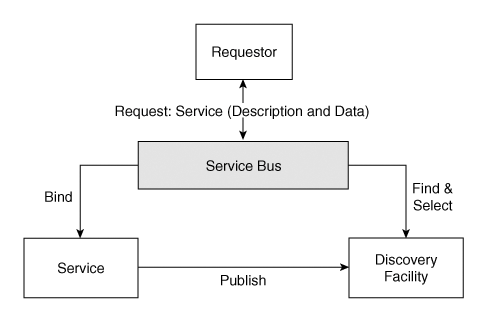
\includegraphics[clip, scale=0.7]{./gfx/servicebus.png}
%	\caption[The Role of the service bus in SOA]{The Role of the service bus in \ac{SOA} \cite{Weera2005} }
%	\label{fig:servicebus}
%\end{figure}

%(see Figure \ref{fig:servicebus})

When receiving a service description (\ac{WSDL}) and data from the service requester, the \ac{ESB} is responsible for selecting the service which best fits to the description requirements, for binding the service requester with the backend service through a route created between the logical endpoints and for making the necessary data transformations to enable the communication between the parts.

As the \ac{ESB} is the central component in \ac{SOA}, and established as integration middleware for services, in this diploma thesis we focus on the required modifications and extensions in the open-source \ac{ESB} Apache ServiceMix 4.3 to provide transparent communication support between the applications and its data located in on-premise databases, or migrated to off-premise data stores. 

\FloatBarrier
\section{Multi-tenancy}
\label{sec:specificationmultitenancy}

In this section we detail the multi-tenant requirements the system must fulfill in order to ensure tenant-isolation at two levels: communication and storage. The final prototype must ensure a multi-tenant aware transparent access to data hosted in the Cloud. Although we provide storage support in our system for hosting migrated tenant's data (see Section \ref{sec:systemoverview}), it does not implement a multi-tenant storage model, because this is not a goal in our design. Therefore, we rely on the multi-tenant storage models different Cloud providers implement.

\subsection{Communication Requirements}

The final prototype must not only support a multi-tenant, but also a multi-protocol communication between endpoints. ServiceMix-mt is shipped with the following multi-tenant aware \ac{BC}s: \ac{HTTP}, \ac{JMS}, and E-mail \cite{gomez2012}. However, the existing communication protocols for data transfer purposes leads us to discard the \ac{JMS} and E-mail. \ac{RDBMS}, e.g. MySQL and PostgreSQL, implement their own protocol in their client/server model, at the \ac{TCP} level of the network stack. At the client side the protocol is supported by the native drivers provided to the developers, e.g. MySQL Connector/J, and at the server side by the different components which build the database server \cite{mysqlmanual}. This fact forces us to provide a vendor-oriented communication protocol environment, by providing support for the different protocols in independent components, rather than in a single standardized component.

Communication in, and from the \ac{ESB} must be multi-tenant aware. We divide the required isolation between tenants into the following sub-requirements: 

	\begin{itemize}
		\item \textbf{Tenant-aware messaging}: messages received in the \ac{ESB} and routed between the tenant-aware endpoints should be enriched with tenant and user information. 
		\item \textbf{Tenant-aware endpoints}: in ServiceMix-mt tenants pack a common endpoint configuration packed in a \ac{SU}, which is then deployed as a \ac{SA} in ServiceMix-mt's \ac{JBI} container \cite{gomez2012}. The multi-tenant aware \ac{BC} dynamically modify the endpoint's URL by injecting tenant context in it. In a database system in our scenario we do not have only tenants as the main actors, but also the different users which can access a tenant's database. Therefore, the tenant-aware endpoints should be dynamically created by injecting tenant and user information in the endpoint's URL. Furthermore, we must ensure tenant and user authentication in the system. 
		\item \textbf{Tenant-aware routing and context}: the deployment of tenant-aware endpoints should be followed by the creation of a tenant-aware context. Resources involved in a routing operation from one consumer endpoint to one provider endpoint can be shared between different tenants, but they must manage the routing operations in different tenant-aware contexts. The routing operations between two endpoints must identity the tenant and user who initiated the routing. 
		\item \textbf{Tenant configuration isolation}: configuration data persisted in our system should be isolated between tenants. A tenant's endpoint configuration data contains sensible information which identifies and allows access to the tenant's backend data stores. 
		\item \textbf{Tenant-aware correlation}: in a request-response operations, the response obtained from the backend data store must be correlated with the tenant's request to the system, and ensure that one tenant does not receive responses from another tenant's request.
	\end{itemize}

\subsection{Storage Requirements}

Due to the fact that our system does not primarily requires multi-tenant aware storage support, but we rely on multi-tenant aware storage systems in the Cloud, we summarize the main requirements for isolating data between tenants in database systems. 

Curino et al. identify as a primary requirement for a Cloud provider offering a \ac{DBaaS} model security and privacy \cite{relationalcloud2010}. A system running multiple database servers and each server multiple database instances must contain the necessary meta-data to provide tenant-aware routing in the system, and ensure that one tenant can only access the information in his database instance. Furthermore, privacy of stored data between tenants can be ensure by encrypting all tuples \cite{relationalcloud2}. Curino et al. introduce \term{CryptDB}, a subsystem of a relational Cloud which provide data encryption and unencryption functionalities for persisting data, and for accessing data via \ac{SQL} queries which are not aware of the encrypted storage mechanism in the system. However, it is known that the key challenge in managing encrypted data in the Cloud is doing it efficiently.

\FloatBarrier
\section{Java Business Integration}
\label{sec:jbi}

The interaction between enterprises' applications has suffered in the past from lack of standardized technologies, leading each of the enterprises to develop their own or acquiring vendor-specific integration technology. \ac{JBI} is defined by the Java Community as an integration technology which maximizes the decoupling between components and defines an interoperation semantic founded on standards-based messaging. This allows different vendor-specific components to interoperate in a multivendor "echosystem" \cite{JBI2005}. 

The key which leads to the integration of different components relies on a unique message format in the \ac{JBI} environment which different plugged-in components use to communicate within the environment. External components are not directly connected, but through a mediator. The communication mediator between components in a \ac{JBI} environment is the \ac{NMR}. Its main functionality is the routing of the internal standardized \ac{NM} between the components. However, it can perform additional processing during the message exchange. The \ac{NMR} fields are defined as an \ac{XML} document format payload, metadata conforming the header and a non \ac{XML} document format attachment referenced by the payload.

The \ac{JBI} specification defines two different types of components which are categorized in two types and provide different services:
	\begin{itemize}
		\item A \ac{SE} provides transformation and composition services to other components.
		\item A \ac{BC} provides the connectivity between the external services and the \ac{JBI} environment. They support many different protocols and isolate the \ac{JBI} environment by marshaling and demarshaling the incoming or outgoing message into the internal standardized \ac{NM} format.
	\end{itemize} 
	
Both components listed above can function as service consumers or service providers following a \ac{WSDL}-based, service-oriented model. The consumer endpoint provides a service accessible through an endpoint which can be consumed by other components, while the provider endpoint consumes a functionality exposed as a service and accessible through an external endpoint. The routing of \ac{NM} starts when a message exchange between components is created (bidirectional communication pipe, a \term{DeliveryChannel}, between the communicating endpoints) and continues with the target of the specified service endpoint for processing (see Figure \ref{fig:jbi}). The \ac{NMR} supports four asynchronous message exchange patterns differing in the reliability and direction of the communication.

\begin{figure}[htb]
	\centering
		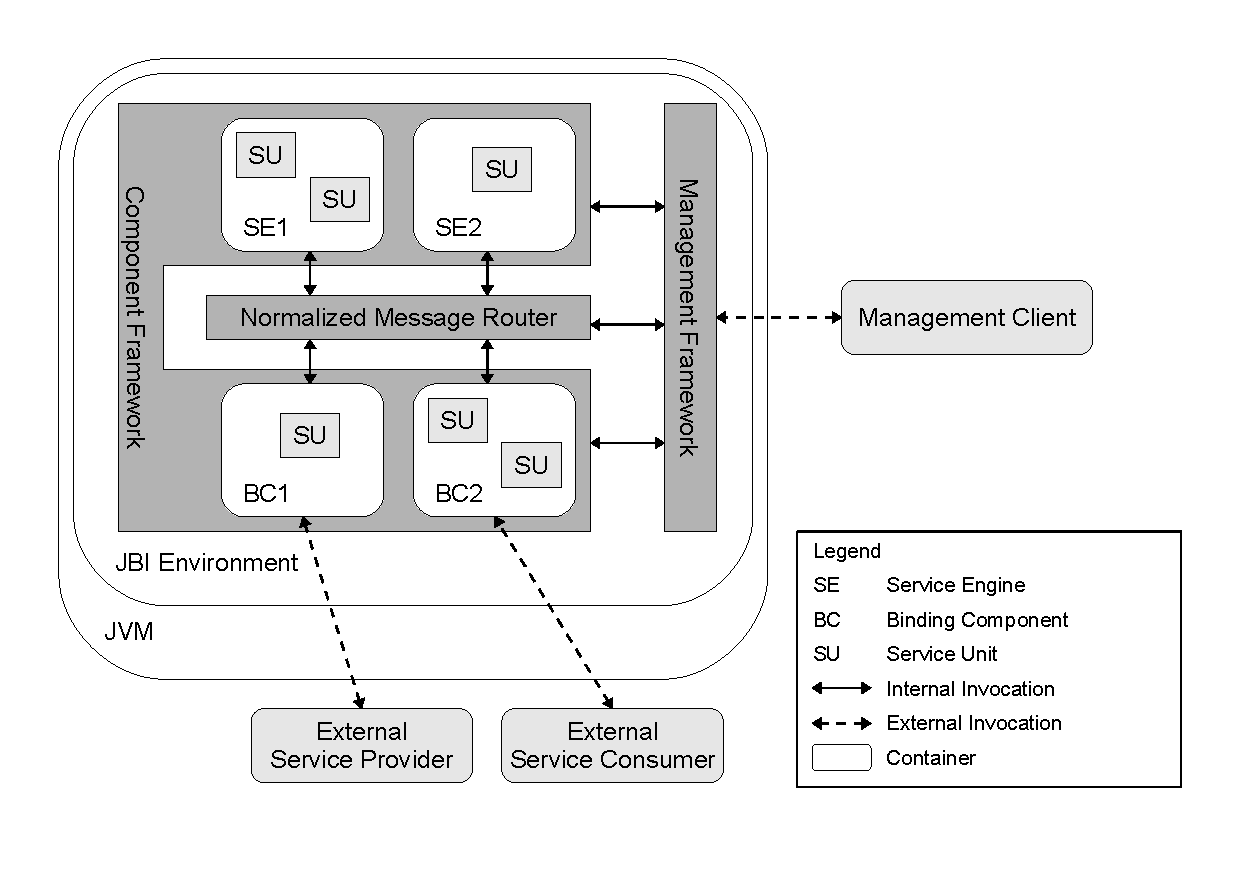
\includegraphics[width=0.85\textwidth, trim=0.95cm 0.95cm 0.95cm 0.95cm, clip]{./gfx/JBIArchitecture.pdf}
	\caption[JBI Architecture]{Overview of JBI Architecture. Figure 4 in JBI specification document \cite{JBI2005}.}
	\label{fig:jbi}
\end{figure}

In Figure \ref{fig:jbi} we can observe that one or more \ac{SU} are contained in a \ac{BC}. The \ac{SU}s are component-specific artifacts to be installed to a \ac{SE} or a \ac{BC} \cite{JBI2005}. The service units are packed in a \ac{SA}, usually as ZIP files, where it is specified each of the components where each of the \ac{SU}s should be deployed. The \ac{JBI} environment provides a Java Management Extension \ac{JMX} Framework for installation, life cycle management, addition, and monitoring and control of the components conforming to the environment defined by the JBI specification.

\FloatBarrier
\section{OSGi Framework}
\label{sec:osgi}

The \ac{OSGi} framework provides loose coupling between modules in a Java environment. It provides a strong support for module versioning and third party modules referencing. The \ac{OSGi} defines a framework for deployment support in a \ac{JVM} of downloaded or extended resources known as \term{bundles}. This framework requires OSGi-friendly devices a minimum system's resources usage by providing dynamic code-loading and \term{bundle} lifecycle management. An \ac{OSGi} \term{bundle} is the packaging of a group of Java classes and required and provided capabilities' meta-data as a JAR file for providing functionality to end users, which can be exposed as bundle services or just run internal processes. A valid \ac{OSGi} bundle can be installed in any valid \ac{OSGi} container due to the standardized packaging and bundle management. 

\ac{OSGi} \term{bundles} can be downloaded, extended and installed remotely or locally in the platform when needed without the need of system reboot. Installation and update of bundles during their lifecycle are also managed by the framework, which uses a service registration for selection, update notifications, or registry of new service objects offered by a deployed bundle. This feature is the main key for connecting bundles whose's services require during runtime capabilities provided by another bundles. The framework defines a bundle's requirement capability as a dependency.      

The \ac{OSGi} framework defines 5 different layers and a bundle's lifecycle \cite{OSGi2011}. An optional Security Layer provides the infrastructure for deploying and managing applications which must be controlled during runtime. The Module Layer lists the rules for package sharing between the deployed bundles. The lifecycle of a bundle can be modified during runtime through an API provided in the lifecycle layer. The main operations implemented are install, update, start, stop or uninstall. 

Apache ServiceMix 4.3.0 is built on and \ac{OSGi}-based runtime kernel, which provides a lightweight container that enables the deployment of various bundles \cite{openesbaction}. Its architecture and functionalities are described in the following section. 

\section{Apache ServiceMix}
\label{sec:servicemix}  

In this diploma thesis we extend a multi-tenant aware version of Apache ServiceMix 4.3.0, referred to it in this document as ServiceMix. Essl evaluates different available \ac{ESB} solutions in the market, and as output of his work provides a selection decision for extending ServiceMix in order to support multi-tenancy \cite{Essl2011}. As mentioned in Section \ref{sec:multitenancy}, a multi-tenant \ac{ESB} solution in a \ac{PaaS} environment must support tenant-aware communication, and tenant-aware administration and management. The support is provided by Muhler and Gomez in their corresponding works in \cite{Muhler2012}, \cite{gomez2012}, leading to a multi-tenant ServiceMix prototype supporting different communication protocols. We will refer to it as ServiceMix-mt.

As a main difference with previous versions' architectures, ServiceMix is an integration container based on the \ac{OSGi} Framework implementation Apache Karaf  \cite{Karaf2011}. It provides a light environment in which components and applications can be deployed in a loose coupled way. Apache Karaf provides an extensible management command line console where management of the components lifecycle, such us \ac{OSGi} bundles, \ac{JBI} components or \ac{SA}s, can be done in a user friendly way (see Figure \ref{fig:servicemix}). Furthermore, a hot deployment directory is shipped with the \ac{ESB} package where users can deploy \ac{OSGi} bundles, \ac{JBI} components wrapped in \ac{SA}'s, etc. just by copying the file into it. The undeployment is done automatically when the user deletes the file from the \term{deploy} directory. 

The main advantage in the ServiceMix 4.3.0 it is its full compliance with the \ac{JBI} specification. Its \ac{JBI} container has as its main component the \ac{NMR} (See Figure \ref{fig:servicemix}). In the \ac{JBI} container users are provided with \ac{JBI} deployment support and management. The communication between the \ac{JBI} and \ac{OSGi} container, e.g. from one \ac{OSGi} service to a \ac{JBI} Binding Component can be achieved through the \ac{NMR} using its API wrapped as an already deployed \ac{OSGi} bundle. This fact eases the integration process of components between different ServiceMix's versions, and take advantage of it in this diploma thesis. Furthermore, \ac{JBI} components or endpoint configurations packed as \ac{SE} or \ac{SA} and deployed in ServiceMix are internally packed into \ac{OSGi} bundles. 

ServiceMix is shipped with different \ac{JBI} components already deployed as \ac{OSGi} bundles in its \ac{OSGi} container. In this thesis we will concentrate on the following ones: HTTP and Apache Camel. Apache Camel is a powerful open source integration framework based on \ac{EAI} \cite{Camel2011}. Furthermore, it provides a widespread list of components which support different communication protocols.  The user can configure logical endpoints between \ac{BC}s and different routing paths between them by deploying their configuration wrapped in a \ac{SA} in the \term{deploy} directory. Different Maven plugins can make the configuration of a \ac{JBI} or \ac{SE} as simple as possible by providing different built archetypes which generates the \ac{SU} files and directories where the developer can configure the component \cite{MAVEN}. Apache Camel provides a set of maven archetypes which already contain the structure for developing custom camel components.

\begin{figure}[htb]
	\centering
		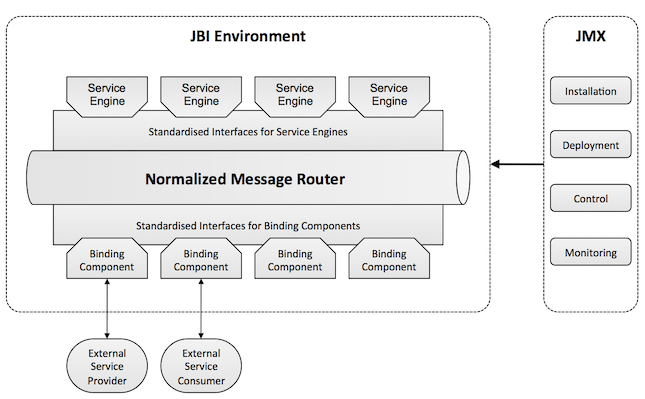
\includegraphics[clip, scale=0.4]{./gfx/servicemix.png}
	\caption[Architecture of Apache ServiceMix]{Architecture of Apache ServiceMix \cite{ASM} }
	\label{fig:servicemix}
\end{figure}

The \ac{NMR} routes the messages between the endpoints created by the \ac{JBI} components (see Figure \ref{fig:servicemix}). This endpoints are divided in two types: consumers and providers. A consumer endpoint is exposed as a service while a provider endpoint consumes an external service. When a message arrives to a consumer endpoint of a \ac{JBI} Binding Component, it is transformed into a \ac{NMF}. The \ac{NMF} is the protocol neutral format which is routed in a \ac{JBI} environment and described in Section \ref{sec:jbi}. 

The ServiceMix-mt prototype we extend in this diploma thesis already provides multi-tenant support for different communication protocols: HTTP, JMS, and E-mail. However, the data retrieval and storage in an application's architecture relies on one specific layer: Data Access Layer, and its main used communication protocols for data transfer are in most of the cases vendor specific. Communication with \ac{SQL} databases, such as MySQL, Oracle, and PostgreSQL are managed by its vendor-specific native driver, which implements the communication protocol with the database server in the \ac{DBMS}. Such protocols are not supported in the multi-tenant prototype ServiceMix-mt, and must be taken into account in the extension of the prototype in this diploma thesis. On the other hand, communication with \ac{NoSQL} databases can be also considered vendor-specific, because most of the Cloud storage providers facilitate its own API to the users to manipulate data in their data containers, but almost all of them provide either REST or \ac{SOAP} over \ac{HTTP} interfaces. This fact permits us to reuse and extend the multi-tenant HTTP \ac{BC} in ServiceMix-mt. The components we create or extend in this diploma thesis are identified by CDASMix (Cloud Data Access Support in ServiceMix-mt).

\FloatBarrier
\section{Binding Components}
\label{sec:bindingcomponents}  

In this section we describe the \ac{JBI} \ac{BC}s shipped in the ServiceMix-mt prototype this diploma thesis focuses on, and the transport protocols they support. 

\subsection{Multi-tenant HTTP Binding Component}

ServiceMix provides \ac{HTTP} communication support in its \ac{HTTP} \ac{JBI} \ac{BC}. Its \ac{HTTP} consumer and provider endpoints are built on the \ac{HTTP} Jetty 6 server and Jakarta Commons \ac{HTTP} Client respectively, providing support for both REST and SOAP over HTTP 1.1 and 1.2 requests.

The original \ac{HTTP} \ac{BC} is extended in the ServiceMix-mt prototype to provide multi-tenant support in \cite{Muhler2012} and \cite{gomez2012}. Muhler provides an internal dynamic creation of tenant-aware endpoints in the \ac{BC}, by injecting tenant context in the \ac{JBI} endpoint's URLs \cite{Muhler2012}. Gomez provides a \ac{NMF} with tenant context information in its properties for routing in the \ac{NMR} \cite{gomez2012}. However, in this diploma thesis we must not only provide tenant isolation at the tenant level, but also isolation at the user level. We discuss this requirement in detail in Chapters \ref{chap:spec} and \ref{chap:design}.

\begin{figure}[htb]
	\centering
		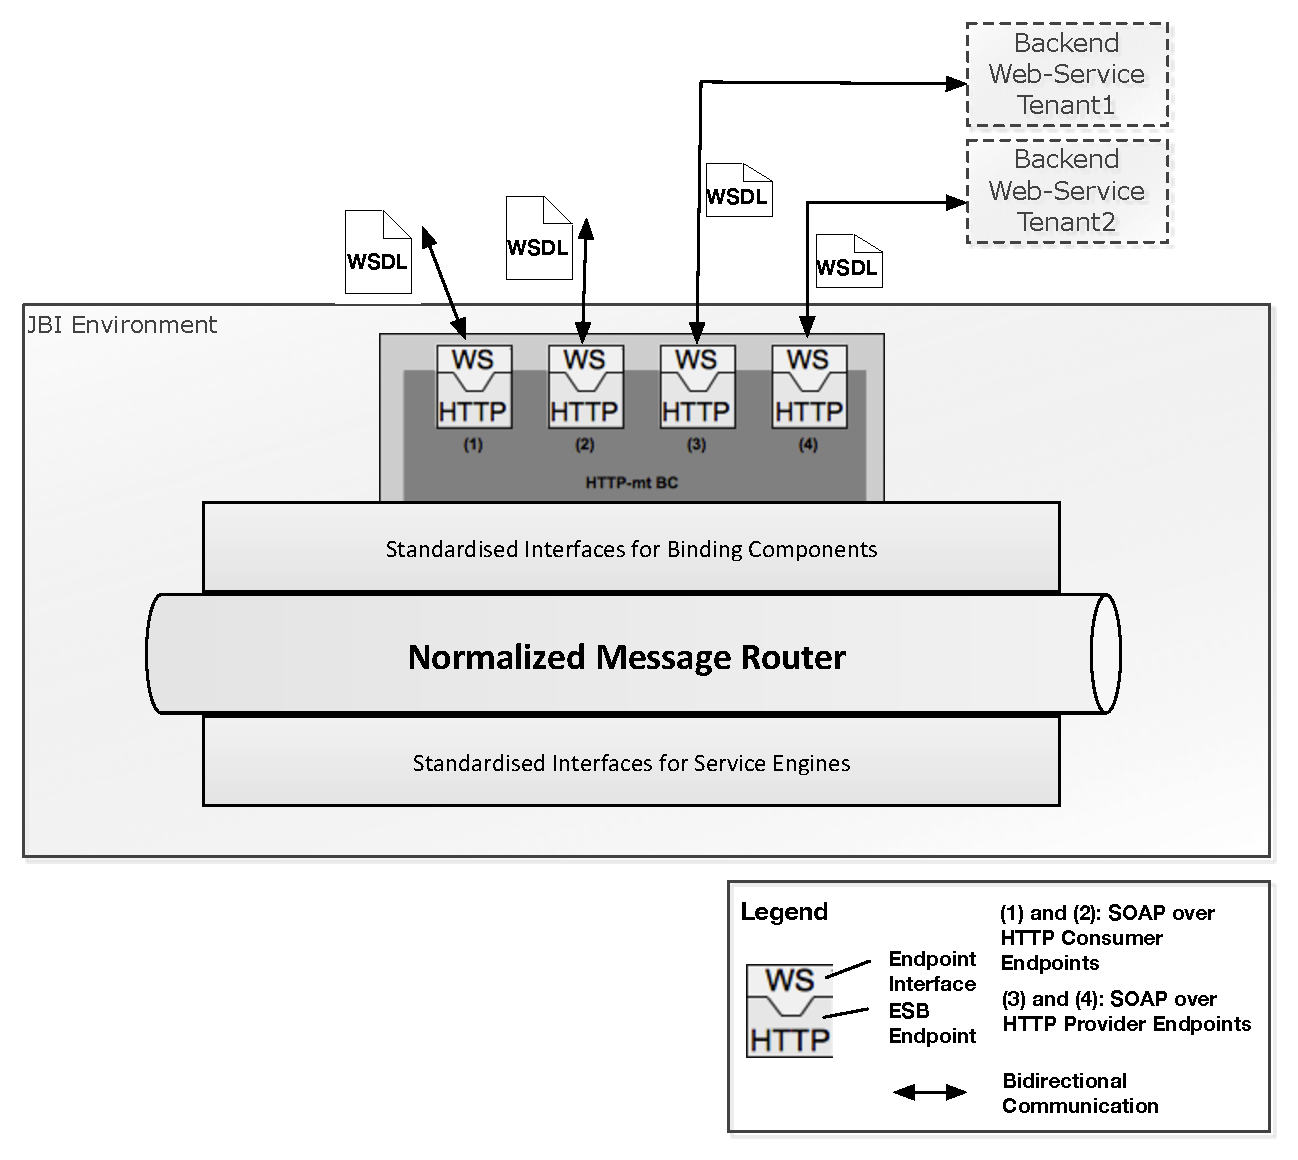
\includegraphics[clip, scale=0.3]{./gfx/httpmtbc.pdf}
	\caption[Multi-tenant HTTP Binding Component]{Multi-tenant HTTP Binding Component \cite{gomez2012}. }
	\label{fig:httpmt}
\end{figure}

As seen in Figure \ref{fig:httpmt}, the multi-tenant \ac{HTTP} \ac{BC} is mainly used in ServiceMix-mt to support the \ac{SOAP} over \ac{HTTP} communication protocol by exposing a Web service in the tenant-aware consumer endpoint and consuming an external Web service in the provider endpoint. \ac{SOAP} defines an \ac{XML} message format  which is sent over the network and a set of rules for processing the \ac{SOAP} message in the different \ac{SOAP} nodes which build the message path between two endpoints \cite{Weera2005}. A \ac{SOAP} message is a composition of three main elements: a SOAP envelope, header, and body. A SOAP envelope may contain zero or more headers and one body. The header may contain processing or authentication data for the ultimate receiver or for the intermediate nodes through the message is routed. The message payload or business data is included in the SOAP body. SOAP is used as a message framework for accessing Web services in loosely coupled infrastructures \cite{Weera2005}. The Web service consumer specifies the functionality to invoke in the SOAP body. If the Web service functionality has a request-response \ac{MEP}, a SOAP message is used to send the response data when the corresponding operation has been executed successfully or the error data in case an error occurred during execution.

Most of the Cloud storage providers provide an \ac{HTTP} interface to the tenants for data management, retrieval, and storage. In this diploma thesis we extend this \ac{JBI} \ac{BC} in order to provide the tenant a transparent access to his \ac{NoSQL} Cloud data stores.

\FloatBarrier

\section{Service Engine}
\label{sec:serviceengine}  

A \ac{SE} can provide different kinds of services, e.g. business logic, routing, and message transformation. In this diploma thesis we will mainly concentrate on one: Apache Camel \cite{Camel2011}, which is wrapped in a ServiceMix-camel \ac{JBI} \ac{SE} in ServiceMix, and in a ServiceMix-camel-mt \ac{JBI} \ac{SE} in ServiceMix-mt  for multi-tenancy awareness..

\subsection{Apache Camel}

Apache Camel is an open-source integration framework based on known \ac{EIP} which supports the creation of routes and mediation rules in either a Java based Domain Specific Language (or Fluent API), via Spring based XML Configuration files or via the Scala DSL \cite{Camel2011}. In ServiceMix, Apache Camel is shipped in a \ac{JBI} \ac{SE}. The routing or mediation rules between two or more endpoints can be specified in an Spring Configuration file or in a \ac{POJO} file whose's class extends the Apache Camel \term{RouteBuilder} class. Route configurations deployed in ServiceMix must follow the \ac{JBI} compliance: files describing the route configuration must be packed in \ac{SU}, and the latter in a \ac{SA}. Apache Camel provides Maven archetypes which generate the needed route configuration files (in \ac{XML} or \ac{POJO} formats) where the developer can program the route between the different supported endpoints \cite{MAVEN}. The configuration in a \ac{XML} file reduces the configuration complexity to a minimum effort of the developer. However, a configuration in a \ac{POJO} class increases the developing complexity but allows the developer to provide logic, filtering, dynamic routing, etc. In the \term{RouteBuilder} class a developer can access, for example, the header of a \ac{NM} and select the target endpoint dynamically depending on the implemented logic. Furthermore, the routing patterns supported by Apache Camel are the point-to-point routing and the publish/subscribe model. 

The endpoints representation in Apache Camel is based on \ac{URI}. This allows this \ac{SE}s to integrate with any messaging transport protocol supported in the \ac{ESB}, e.g. \ac{HTTP}, \ac{JMS} via ActiveMQ, E-Mail, CXF, etc. The ServiceMix-camel \ac{JBI} \ac{SE} provides integration support between camel and \ac{JBI} endpoints. Muhler extends this component and allows dynamic internal creation of tenant-aware endpoints in the ServiceMix-camel-mt \ac{JBI} \ac{SE} \cite{Muhler2012}. The main goal of this extension is to provide an integrated environment between \ac{JBI} and camel supported endpoints. However, multi-tenancy is supported at the tenant level only in the \ac{JBI} endpoints. In this diploma thesis we aim to enable multi-tenancy not only at the tenant level, but also at the user level, as discussed in Chapters \ref{chap:spec} and \ref{chap:design}.

For enabling data access support with \ac{SQL} \ac{DBMS} in ServiceMix-mt we extend a well-known camel component: Camel-jdbc. The Camel-jdbc component enables \ac{JDBC} access to \ac{SQL} databases, using the standard \ac{JDBC} API, where queries and operations are sent in the message body \cite{cameljdbc}. This component requires the developer to statically denote the data source configuration (user, password, database name, etc.) in both the endpoint \ac{URI} and route configuration file. As discussed in Chapters \ref{chap:spec} and \ref{chap:design}, this requirement is opposite to our approach, due to the dynamism we need in creating connections to the different \ac{DBaaS} providers. We extend and produce a custom camel component: Camel-jdbccdasmix (\term{cdasmix} stands for Cloud Data Access Support in ServiceMix-mt).

\FloatBarrier

\section{SQL Support Architectural Overview}
\label{sec:designsql}

In this section we provide an overview of a preliminary, and final architectural approaches designed in this diploma thesis, in order to support a transparent data access to backend \ac{SQL} databases. We first expose the integration approaches we should consider, and the main problems found when implementing the first approach which led us to design a second architectural approach. 


\subsection{Integration}

%integration of osgi and jbi in terms of messaging
%integration of osgi and jbi in terms of containers and libraries
%explain why we have two approaches
%jbi components offered in servicmix are deployed as osgi bundles
% jbi components offered in servicemix-mt are deployed as jbi component, and internally wrapped into an osgi bundle
% may have to put a figure of the contents in both of the packages so that we can see. It is all about the meta inf library where the bundle manifest info is exposed
As described in Chapter \ref{chap:spec}, we build the new components in ServiceMix-mt following the \ac{OSGi} compliance. However, these must interact with components which follow the \ac{JBI} specification. The integration between components built for different containers in ServiceMix-mt must be done at two levels: messaging, and resources sharing. The ServiceMix-mt \ac{NMR} \ac{API} \ac{OSGi} bundle exposes a set of operations for sending messages through the \ac{NMR} to a specified target endpoint. Hereby we can perform message exchanges between endpoints configured on \ac{OSGi} bundles and endpoints configured on \ac{JBI} components, and provide communication support between components hosted in the two containers. 

\begin{figure}[htb]
	\centering
		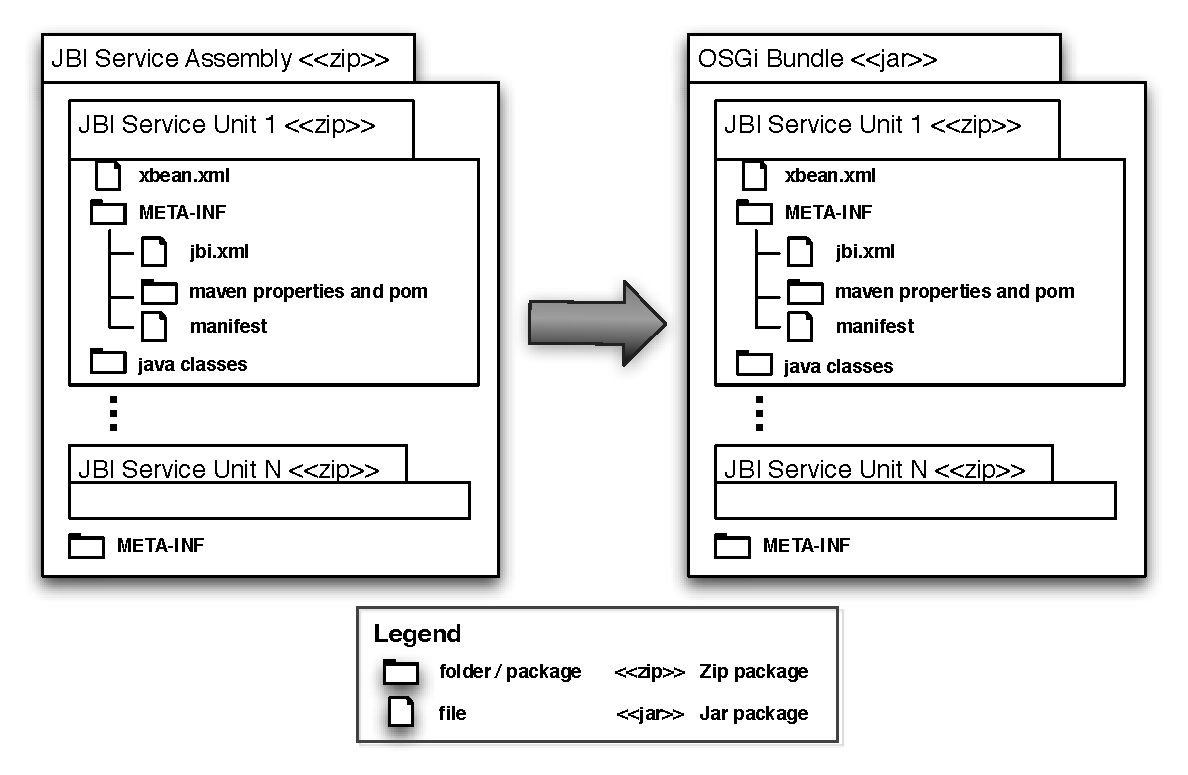
\includegraphics[clip, scale=0.5]{./gfx/osgibundlepackage.pdf}
	\caption[JBI to OSGi repackaging]{ServiceMix 4.x repackaging mechanism for deploying \ac{JBI} components in \ac{OSGi} container.}
	\label{fig:jbitoosgipackage}
\end{figure}

The resources sharing integration level refers to the deployment of \ac{JBI} components in the \ac{OSGi} container, and the utilization of packages exposed by \ac{OSGi} bundles in the \ac{OSGi} container in a loosely coupled manner. The former is part of the integration between containers provided in ServiceMix 4.x versions and described in Figure \ref{fig:jbitoosgipackage}. The deployment mechanism of a \ac{JBI} \ac{SA} into an \ac{OSGi} container is simple: repackaging of the \ac{SA} as a JAR. However, this cannot be consider a full integration in the \ac{OSGi} container. \ac{OSGi} bundles contain in their \term{META-INF} folder one fundamental file for the \ac{OSGi} kernel: the \term{manifest} file. This contains a description of the bundle, the packages it imports, and exports. Imported packages can be either statically stored in the bundle or imported from third party bundles, and exported packages are the ones which exposed to third party bundles. These can be imported with an internal class loading mechanisms developed in the \ac{OSGi} container. The repackaging of the \ac{SA} into a JAR, as it is shown in Figure \ref{fig:jbitoosgipackage}, contains the \term{META-INF} folder, and the \term{manifest} file. However, the latter only contains information about the author, date of creation, but it does not contain information related to the exported packages, and the needed packages to be imported. This \term{manifest} file describes the \ac{SA}, and not the \ac{SU}s. Java classes and package importing description are contained in the \ac{SU} package, and not in the \ac{SA} package. Therefore, the \ac{OSGi} container cannot register in its registry the packages it exports as a service, and cannot load the imported packages to the bundle context. This fact forces us to statically include in the \ac{SA}, and the \ac{SU} the packages which are referenced in each \ac{SU}, and leads to scalability constraints with the tenant-aware deployment process of the system.

ServiceMix 4.x versions are shipped with different \ac{JBI} \ac{BC}s packed as an \ac{OSGi} bundle. However, they are deployed as \ac{OSGi} bundles, and not as \ac{SA}s, in order to enable loose coupling and package sharing between components in the \ac{OSGi} container. ServiceMix-mt allows the deployment of the \ac{JBI} \ac{BC}s, but deployment of \ac{JBI} \ac{BC}s as OSGi bundles is not supported in the JBIMulti2 application. This lack of support forces us to design a second architectural approach, as described in the following sections.

\FloatBarrier

\subsection{Approach 1}

\ac{SQL} database systems provide access to their databases through an endpoint, which is represented as an URL. The native driver used in the data access layer of an application connects to the endpoint, authenticates, sends the query, and reads the response. Therefore, we must support in our system the same operational steps. As discussed in this diploma thesis, the communication protocol varies between different vendors. In this diploma thesis we provide support for incoming MySQL messages. Tenants must access our system through a single physical endpoint. This endpoint is provided by a MySQL proxy which is enriched with authentication, cashing, marshaling, and demarshaling operations. As shown in Figure \ref{fig:designsqlapp1}, the MySQL Proxy Bundle implements the MySQL server operations which are related with the client/server communication protocol. In Figure \ref{fig:designsqlapp1} we specify a server running on port 3306. However, this value can be configured before the deployment of the \ac{OSGi} component. This component is built as an \ac{OSGi} bundle and its packages are exported as services in the \ac{OSGi} container. It interacts with three different components in the system: the \ac{NMR} \ac{API}, the Cache, and the Service Registry. 

Cashing mechanisms are implemented in both the Registry-Cache, and the MySQL Proxy Bundle. The former provides an \ac{API} for creating cache instances, and for persisting and retrieving data. We create a separate cache instance for the \ac{SQL} support due to the need of a custom key creation mechanism which may not coexist in a shared cache between different bundles, as well as the needed isolation of sensible tenant configuration information from third party bundles. The system provides a set of operations which ease the creation of multi-tenant aware keys for persisting frontend authentication data, and queries results form the backend database systems. 

The \ac{NMR} \ac{API} is shipped in ServiceMix as an \ac{OSGi} bundle which exports its \ac{API} as an \ac{OSGi} service. The set of operations included in its \ac{API} allows \ac{OSGi} bundles to create, send, and receive message exchanges to \ac{JBI} endpoints (see Figure \ref{fig:designsqlapp1}).  Before creating the message exchange, the MySQL Proxy Bundle must build dynamically the target endpoint's URL by injecting the tenant context information, and service and endpoint name.

\begin{figure}[htb]
	\centering
		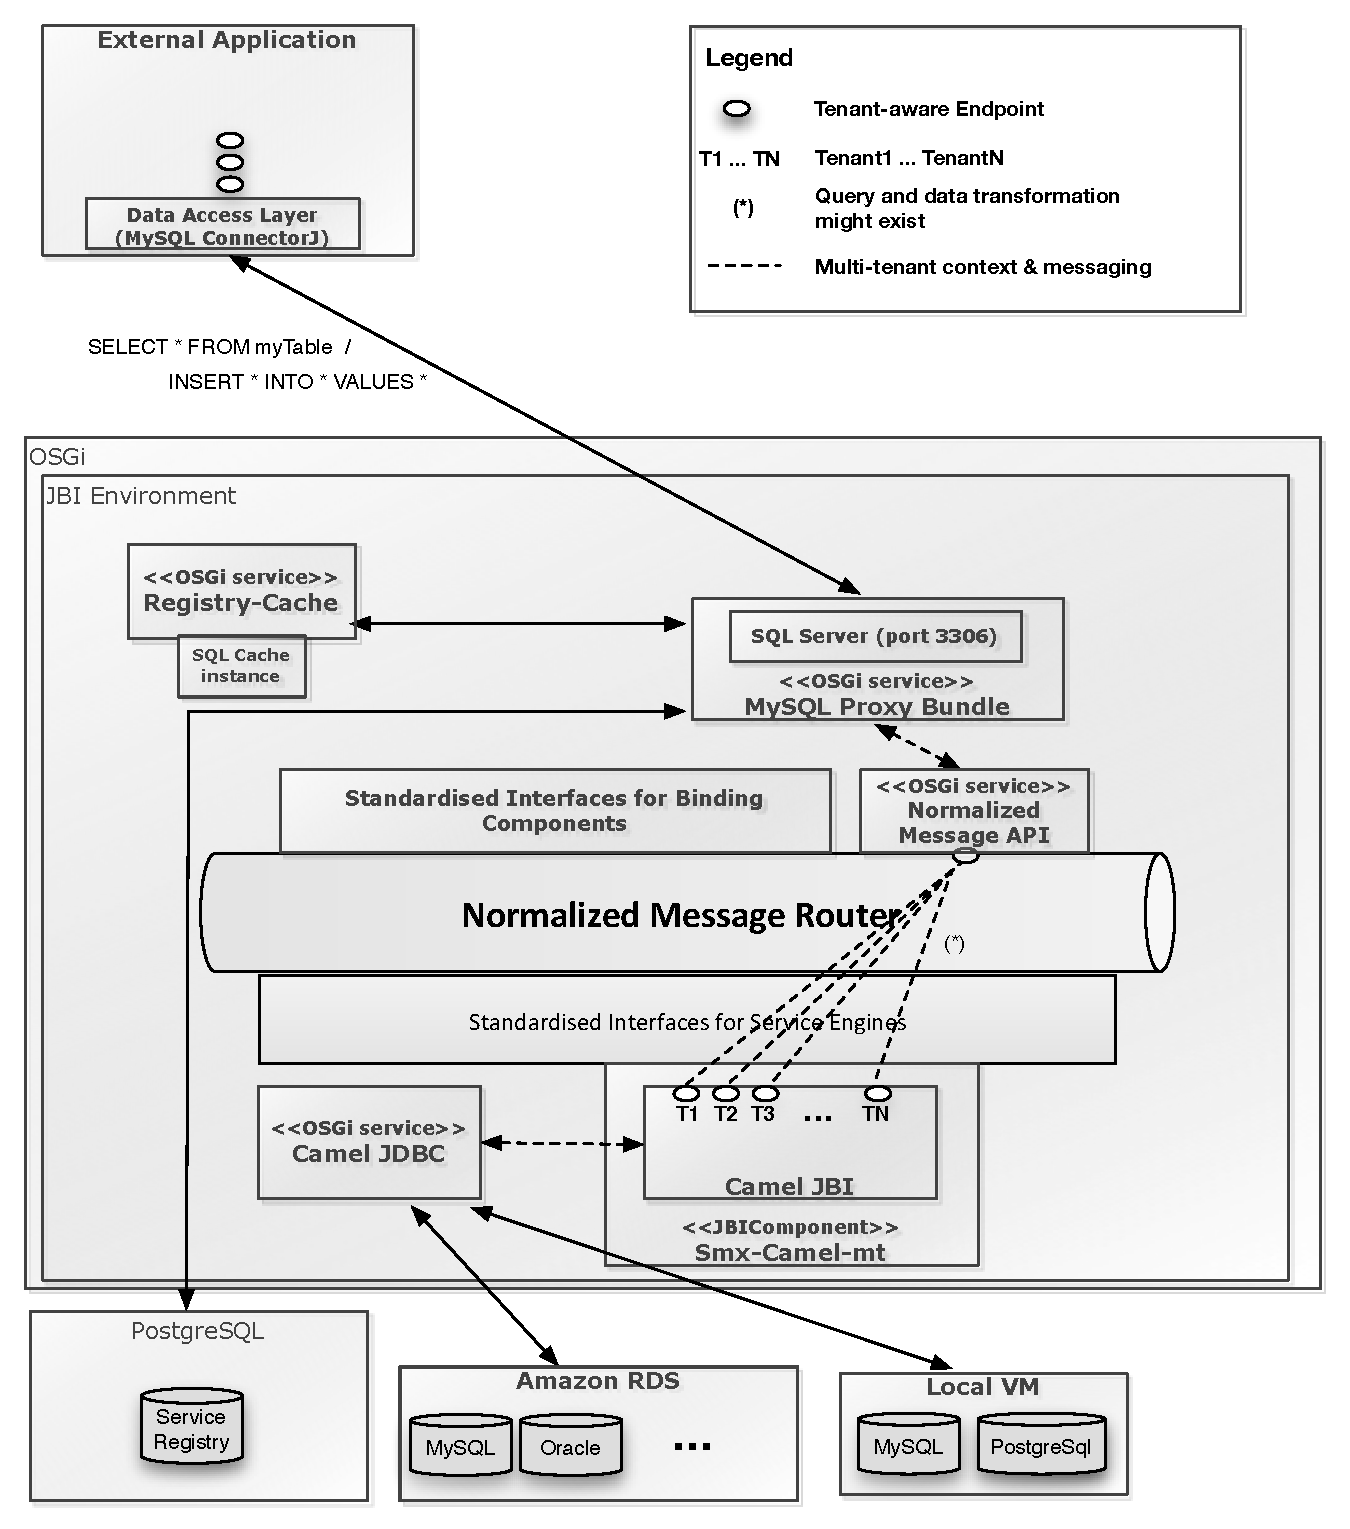
\includegraphics[clip, scale=0.6]{./gfx/sqlApproach/sqlApproachv2_doc.pdf}
	\caption[SQL Support Approach 1]{Architectural overview of the design approach one to support the MySQL communication protocol and routing to backend \ac{SQL} databases.}
	\label{fig:designsqlapp1}
\end{figure}

Apache Camel provides a set of components which integrate most of the communication technologies available in the market. Moreover, it provides an archetype for creating custom components we use in this diploma thesis. ServiceMix provides a Camel \ac{JBI} \ac{BC} which integrates the \ac{JBI} container with the camel router. Muhler extends this component in ServiceMix-mt and enriches it with multi-tenancy awareness. However, the supported multi-tenancy is at the level of tenants, and not at the level of tenant's users. We extend this component and provide user and tenant isolation between endpoints, by injecting the tenant and user UUID in the endpoint's URI (see Listing \ref{lst:endpointuri}). 

%%%%%%%%%%%%%%%%%%%%%%%%%%%%%
\lstinputlisting[float=htb,label={lst:endpointuri},caption={[Tenant-aware Endpoint Configuration]Extended Tenant-aware endpoint URI in extended Backus-Naur Form (EBNF) \cite{Muhler2012}.},style=ebnf]{./gfx/endpointconfiguration.txt}
%%%%%%%%%%%%%%%%%%%%%%%%%%%%%

With multi-tenancy at the tenant and user level, each user can deploy one \ac{JBI} tenant-aware endpoint in the ServiceMix-Camel-mt \ac{SE}. The routes deployed from each tenant-aware endpoint are performed under a different context, and an instance of the targeted component in the route is created. Therefore, with this approach we provide multi-tenancy at the messaging, endpoint, and routing and component context levels. 

Due to the lack of \ac{JDBC} support in ServiceMix for creating provider endpoints, we develop a custom camel component, and enrich it with \ac{JDBC} support for three database systems: MySQL, Oracle, and PostgreSQL. This component is extensible to more database systems when including its native driver, and is build as an \ac{OSGi} bundle and its packages are exported as an \ac{OSGi} service. Messages received from the \ac{NMR} are demarshaled to the backend database system communication protocol, and the response marshaled, correlated, and sent back to the MySQL Proxy Bundle. The demarshalers in this bundle provide the necessary support for transforming the \ac{NMF} response to a MySQL message.

As described in the previous section, ServiceMix-mt provides \ac{JBI} and \ac{OSGi} support and integration, but with some constraints. \ac{JBI} components cannot import packages from \ac{OSGi} bundles exporting its packages. The Servicemix-Camel-mt \ac{SE} provides integration with the camel router for a set of camel components. The camel manual specifies the need for adding statically the custom component packages in the \ac{JBI} \ac{SU} which contains the route definition. Therefore, this leads us to scalability problems in each of the \ac{SA} deployed by the tenants. The \ac{SA} size increases with the new supported database systems, and forces to redeploy all the \ac{SU}s containing the custom camel component when it is modified. This leads to management, storage capacity, and network capacity inconveniences. Hence, we provide a second, and final approach which is very similar to this one, but utilizing the ServiceMix-camel component deployed as \ac{OSGi} bundle. 

\FloatBarrier

\subsection{Approach 2}

In this second architectural design approach we address the scalability problems caused by the \ac{JBI} package dependencies in the \ac{SU}s described in the previous section. This approach is similar to the first one presented, and its main difference relies on the routing from the tenant-aware \ac{JBI} endpoints to the custom camel component \term{cdasmixjdbc} (see Figures \ref{fig:designsqlapp2} and \ref{fig:designsqlapp1}). The functionalities and operations in the MySQL proxy bundle do not differ with the previous approach.
 
\begin{figure}[htb]
	\centering
		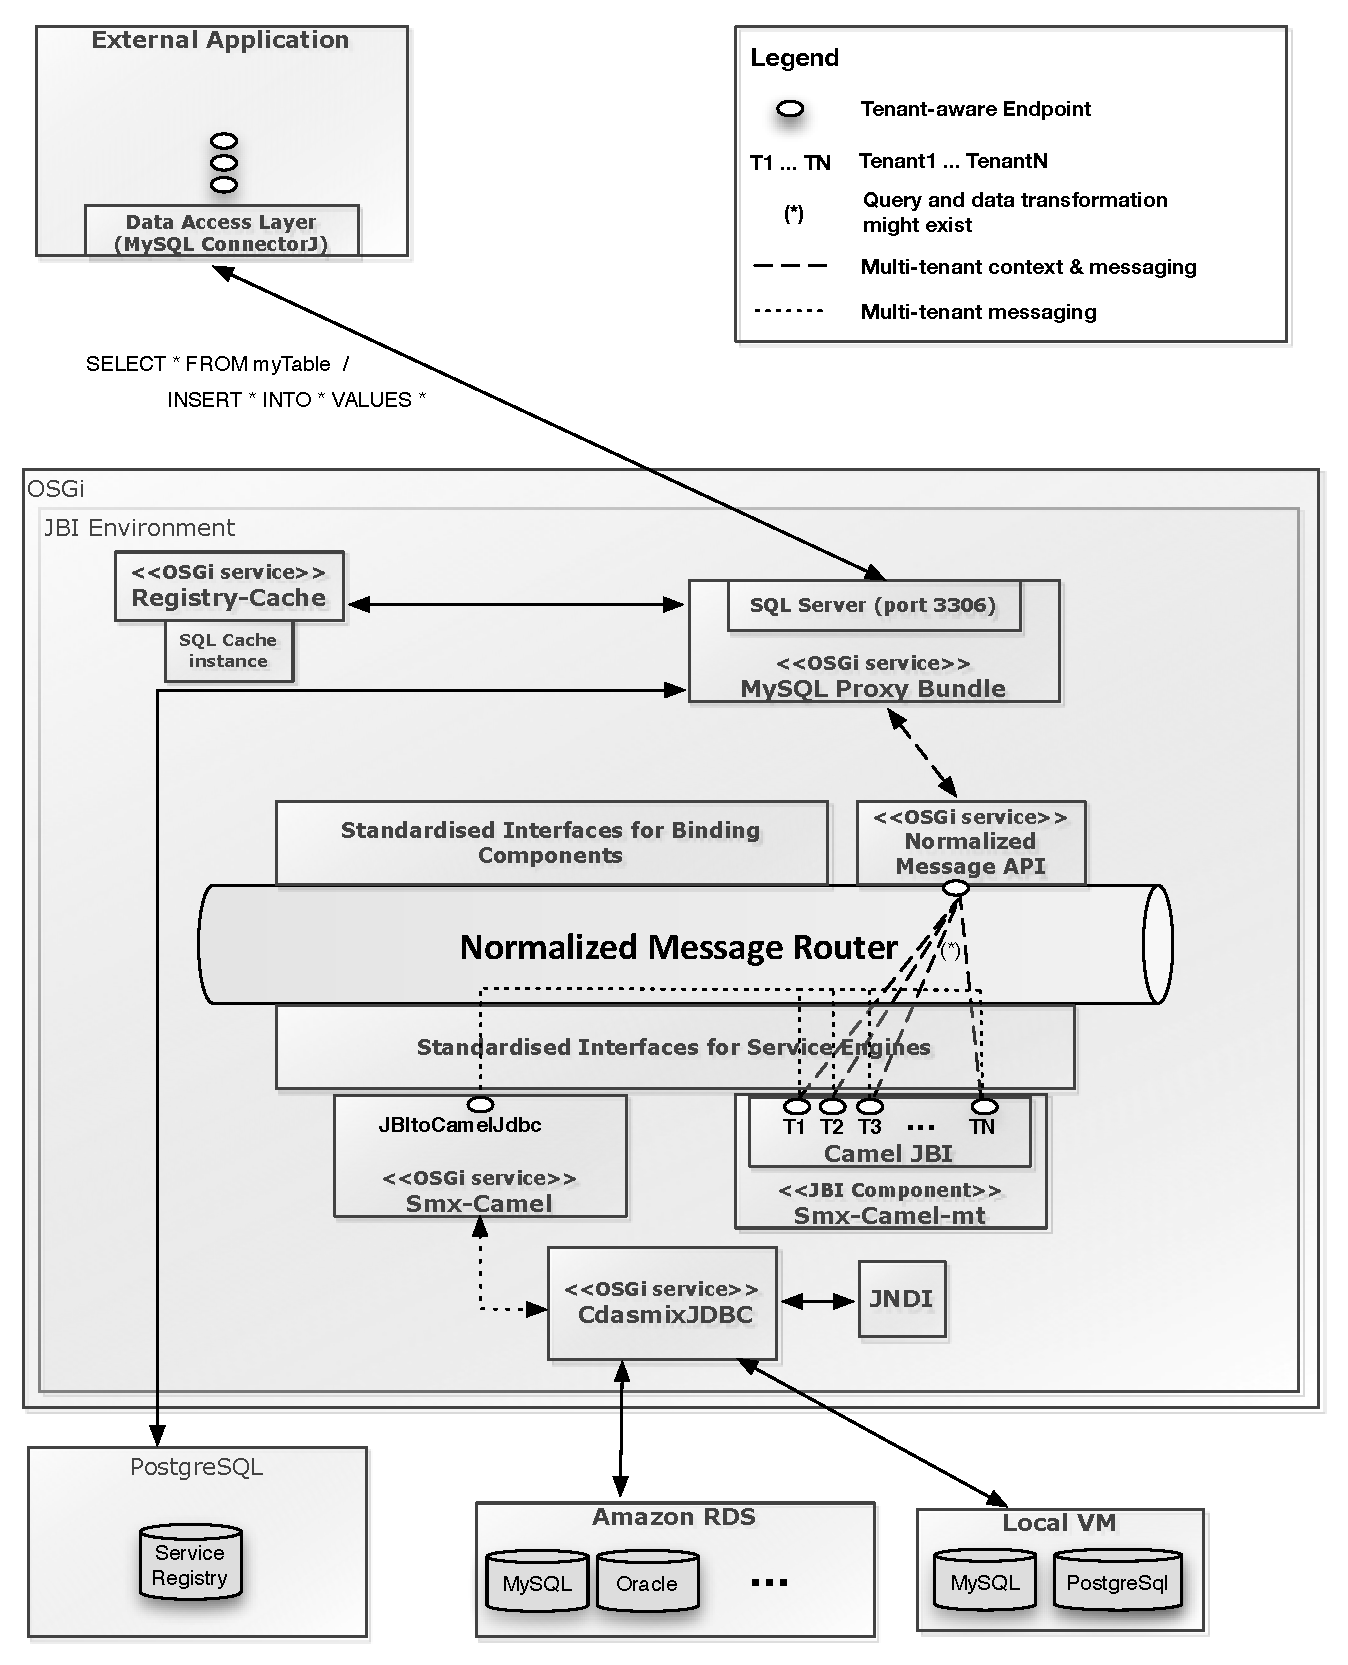
\includegraphics[clip, scale=0.6]{./gfx/sqlApproach/sqlApproachv3_doc.pdf}
	\caption[SQL Support Approach 2]{Architectural overview of the design approach two to support the MySQL communication protocol and routing to backend \ac{SQL} databases.}
	\label{fig:designsqlapp2}
\end{figure}

The message is routed from the MySQL proxy bundle to the tenant-aware \ac{JBI} endpoint deployed in ServiceMix-camel-mt. The multi-tenant message processor instance in ServiceMix-camel-mt routes the message to the \term{JBItoCamelJdbc} endpoint. 

As discussed before, the \ac{JBI} \ac{BC}s deployed in ServiceMix are \ac{OSGi} friendly. This means that the \ac{OSGi} contains a valid manifest file where the description of the bundle, import packages, and export packages are specified. \ac{SU}s deployed on this component are able to reference other \ac{OSGi} packages exposed as a service in the \ac{OSGi} service registry. We provide a single endpoint deployed in the ServiceMix-Camel component where the requests are sent to: the \term{JBItoCamelJdbc} endpoint. When the \term{JBItoCamelJdbc} endpoint is deployed on the ServiceMix-Camel \ac{OSGi} bundle, this searchs in the \ac{OSGi} container for the \term{CdasmixJDBC} component, and creates an instance of the component. Messages routed to the \term{JBItoCamelJdbc} endpoint are then forwarded to the \term{CdasmixJDBC} component, which selects the appropriate \ac{JDBC} native driver, creates a connection, demarshals the request, and forwards the request to the backend Cloud data store server. The connection is established after creating an instance of a \term{DataSource}, which is saved in the \ac{JNDI} registry for future connections, in order to avoid the creation of more than one \term{DataSource} instance per user per backend Cloud data store.

Responses retrieved from the backend Cloud data store are correlated with the initial request and routed back to the MySQL proxy bundle, which demarshals the retrieved data and sends it as a binary \ac{TCP} stream.

In this approach a new instance of the \term{cdasmixjdbc} is not created per tenant endpoint, but is shared between the tenants. Therefore, we cannot ensure an independent component context at the provider endpoint. However, messages contain the tenant information, and the \term{cdasmixjdbc} component interacts with the backend database system establishing separate \ac{JDBC} connections per request. Full multi-tenancy, at the levels of component creation, and endpoint level is not ensured, but it is ensured at the messaging, and context levels. Although full multi-tenancy is not supported, we avoid the deployment of \ac{SU}s which contain the \term{CdasmixJDBC} component in it, and whose size increase may lead to scalability problems in the system. Furthermore, we prevent the deployment of the same component n times, for the n multi-tenant aware endpoints, and prevent future management problems when modifying or upgrading the \term{CdasmixJDBC} component. 

\FloatBarrier



\section{NoSQL Databases}
\label{sec:fundamentalsnosqldb}  

\ac{RDBMS}s ensure data persistency over time and provide a wide set of features. However, the functionalities supported require a complexity, which is sometimes not needed for some applications, and harms important requirements in Web applications or in \ac{SOA} based applications, e.g. throughput. \ac{NoSQL} data stores aim to improve the efficiency of large amount of data storage while reducing its management cost \cite{nosqlcomputerworld}. NoSQL databases are designed to support horizontal scalability without relying on the highly available hardware \cite{strauchnosql}. In a Cloud storage environment where the user sees the available computing and storage resources as unlimited, a \ac{NoSQL} support in a Cloud storage environment might be adequate.

\ac{NoSQL} \ac{DBS} operate as a schema-less storage system, allowing the user to access, modify or freely insert his data without having to make first changes in the data structure \cite{nosql2012}. Cloud providers provide the users with an \ac{API} for accessing, modifying, and inserting data into his isolated container. For example, a user's Amazon Dynamo DB table and item can be accessed by its RESTful \ac{API}, or by installing at the user's side application the Amazon Web Services SDK \cite{amazondynamodb}. Furthermore, it provides the users through its Web-based management console the available management operations. 

Due to the growth of the \ac{NoSQL} support along different Cloud vendors, in this diploma thesis we provide a multi-tenant and transparent communication support for \ac{NoSQL} backend data stores in different Cloud providers. In the following sections we introduce the categorization of the different \ac{NoSQL} databases we aim to support in this diploma thesis, mentioning and giving examples of Cloud data stores available nowadays in the market.

\subsection{Key-value Databases}

In a key-value datastore elements are uniquely identified by an id, which the data store does not take into account its type, and are simply stored as a \ac{BLOB} . A user can get the value for the key, put a value for the key, or delete a key from the data store \cite{nosql2012}. Its storage model can be compared to a map/dictionary \cite{strauchnosql}. Products offering this data storage model in a Cloud infrastructure are Amazon DynamoDB \cite{amazondynamodb}, Google Cloud Storage \cite{googlecloudstorage}, Amazon SimpleDB  \cite{amazonsimpledb} , Amazon S3 \cite{amazons3}, etc. In this diploma thesis we mainly focus on the following key-value data stores: DynamoDB, and Google Cloud Storage.

Amazon DynamoDB's data model includes the following concepts: tables, items, and attributes \cite{amazondynamodb}. The attributes are a key-value, where the value is binary data. Attributes are stored in items, and these are stored in tables. Items stored in a table can be retrieved by referencing its unique id. The number of attributes is not limited by Amazon, but each item must have a maximum size of 64 KB. Accessing stored data in this data store can be mainly done in two ways: using the functionalities provided by the AWS SDK, or using the Cloud storage RESTful \ac{API}. 

Google Cloud Storage's data model includes the following concepts: buckets and objects \cite{googlecloudstorage}. Buckets contain on or more objects. The objects are identified within a bucket with its unique id. Users can perform I/O operations on both buckets and objects. For this purpose, Google Cloud storage provides RESTful \ac{API}.

In this diploma thesis we use an \ac{ESB} for accessing transparently tenant's databases migrated to the Cloud. Servicemix-mt provides multi-tenant \ac{HTTP} support \cite{gomez2012}. Therefore, we reuse and extend the multi-tenant \ac{HTTP} \ac{BC} in order to provide dynamic routing between the different data stores.

\subsection{Document Databases}

Document databases can be considered as a next step in improving the key-value storage model. In this storage model, documents are stored in the value part of the key-value store, making the value content examinable \cite{nosql2012}. Documents with different schemas are supported in the same collection, and can be referenced by the collection's key or by the document's attributes. One of the main difference in the attributes specification regarding \ac{RDBMS} is that in document stores document's attributes cannot be null. When there is an attribute without value, the attribute does not exist in the document's schema. Products implementing this data storage model are Apache CouchDB, MongoDB, etc. \cite{couchdb} \cite{mongodb}.

Mongo DB defines two storage structures: collections and documents \cite{mongodb}. A specific database contains one or more collections identified by its unique id. A specific collection stores one or more documents. Collections and documents stored in a database can be accessed, inserted and modified using the RESTful \ac{API} supported by the database system.

Apache CouchDB defines two storage structures: databases and documents. Data stored in CouchDB are \ac{JSON} documents. The main difference between this two described databases is that MongoDB implements a two step access to the documents: database, collection, and document. Apache CouchDB provides a RESTful \ac{API} for I/O operations.

This databases are not offered by Cloud providers like Amazon or Google, but as a software which can be deployed in user instances, e.g. Amazon EC2 AMI \cite{amazonec2}. 

\subsection{Column-family Stores}

One of the most known Column-family data stores is Cassandra. Column-family data stores store data in column families (groups of related columns which are often accessed together) as rows that have many columns associated with a row key \cite{nosql2012}. This approach allows to store and process data by column instead of by row, providing a higher performance when accessing large amount of data, e.g. allowing the application to access common accessed information in less time.

Cassandra has as its smallest unit of storage the column, which consists of a timestamp and a name-value pair where the name acts as a key \cite{nosql2012}. As in the relational model, a set of columns form up a row, which is identified by a key. A column family is a collection of similar rows. The main difference with the relational model is that each of the rows must not have the same columns, allowing the designer and the application consuming large amounts of data to customize the columns in each row, and the rows in each column family.

Cassandra is not shipped with a RESTful API for I/O operations. However, there are several open-source services layers for Cassandra, e.g. Virgil \cite{virgil}.

\FloatBarrier

\section{JBIMulti2}
\label{sec:jbimulti2}  

A multi-tenant management system must fulfill several requirements, such as data and performance isolation between tenants and users, authentication, specification of different user roles, resources usage monitoring, etc. In a \ac{JBI} environment, endpoint and routing configurations files are packed in \ac{SU}s, and the latter in \ac{SA}s for deployment. However, there is a lack of user-specific data during deployment. Muhler solves this problem in JBIMulti2 by injecting tenant context in the \ac{SA} packages, making them tenant-aware \cite{Muhler2012}. 

\begin{figure}[htb]
	\centering
		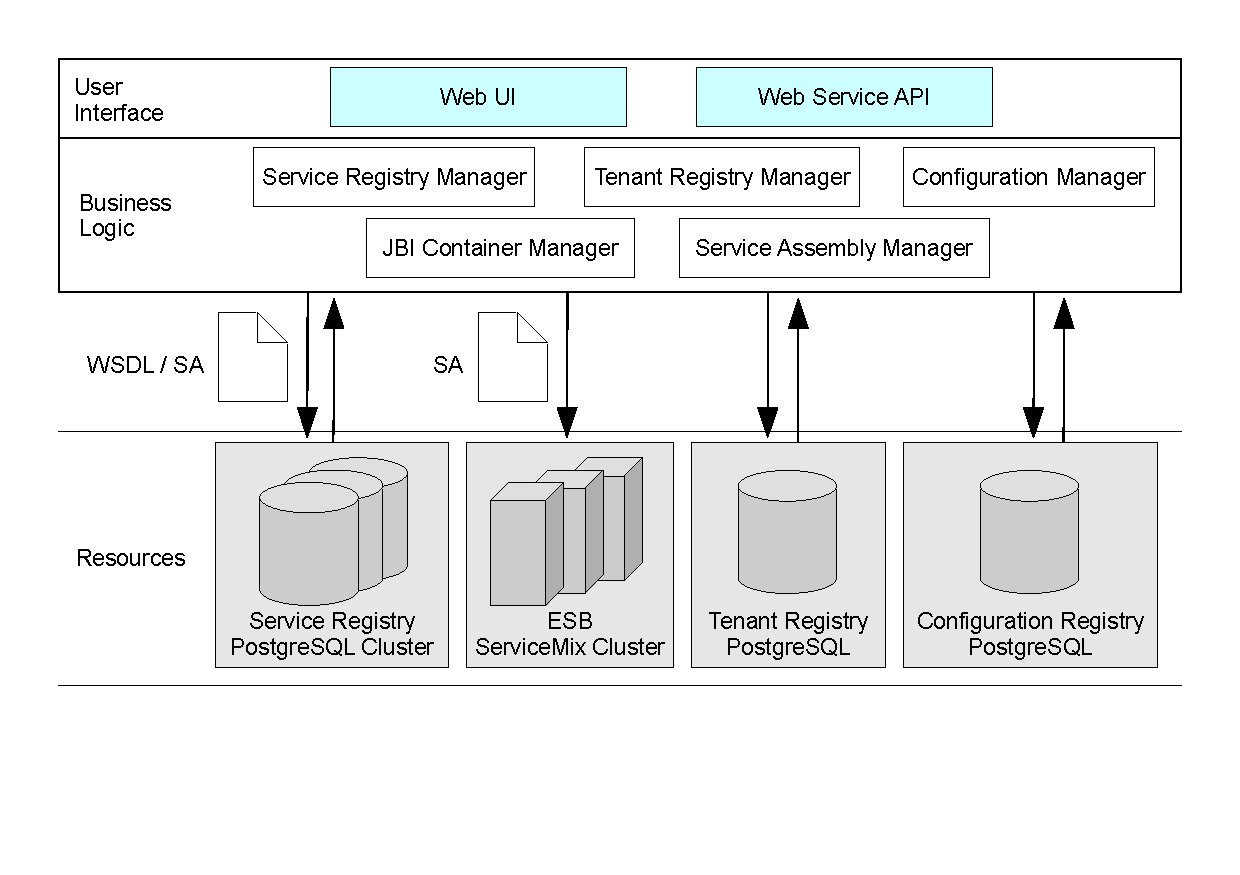
\includegraphics[clip, scale=0.5]{./gfx/systemoverview_jbimulti2.pdf}
	\caption[JBIMulti2 System Overview]{JBIMulti2 System Overview \cite{Muhler2012}} 
	\label{fig:jbimulti2}
\end{figure}

The architecture of the JBIMulti2 system is represented in Figure \ref{fig:jbimulti2}. We can distinguish two main parts in the system: business logic and resources. JBIMulti2 uses three registries for storing configuration and management data. When a tenant (or a tenant user) is registered, an unique identification number is given to them and stored in the Tenant Registry. Both Tenant Registry and Service Registry are designed for storing data of more than one deployed application. The former for storing tenant information and the latter for providing a dynamic service discovery functionality between the different applications accessed through the \ac{ESB}. The Configuration Registry is the key of the tenant isolation requirement of the system. Each of the stored tables are indexed by the tenant id  and user id value. In this thesis we need tenant information during runtime. We reuse and extend the databases schemas produced by Muhler, specifically the Service Registry.

The system provides a user interface for accessing the application's business logic. Through the business logic, the management of tenants can be done by the system administrator or the management of tenant's users can be done by the tenants. Furthermore, when deploying the different tenant's endpoint configurations packed in \ac{SA}s, the system first makes modifications in the zip file for adding tenant context information and then communicates with the Apache ServiceMix instance by using a \ac{JMS} Topic to which all the ServiceMix instances are subscribed to. The \ac{JMS} management service in ServiceMix deploys the received \ac{SA} injected in the received \ac{JMS} message using the administration functionalities provided in ServiceMix. The communication between the business layer and the ServiceMix instance is unidirectional. When successful deployment, the endpoint is reachable by the tenant. When an error occur during deployment, an unprocessed management message is posted in a dead letter queue.

JBIMulti2 requires the previous installation of components, e.g. JOnAS server, PostgreSQL, etc. The initialization of the application is described in both Chapter \ref{chap:validationevaluation} and in the JBIMulti2 setup document \cite{JBIMulti2Man}.
\section{Cloud Data Migration Application}
\label{sec:clouddatamigrationtool}  

The Cloud Data Migration Application provides support to the user before and during the data migration process to the Cloud. It contains a registry of different Cloud data hosting solutions and its properties, which are used during the decision process. The decision process consists in selecting the Cloud provider which best fits the user's operational and economical interests, and in detecting incompatibilities with the selected target data store. The different steps of the migration process are shown in Figure \ref{fig:cloudmigrateapp}. 

\begin{figure}[htb]
	\centering
		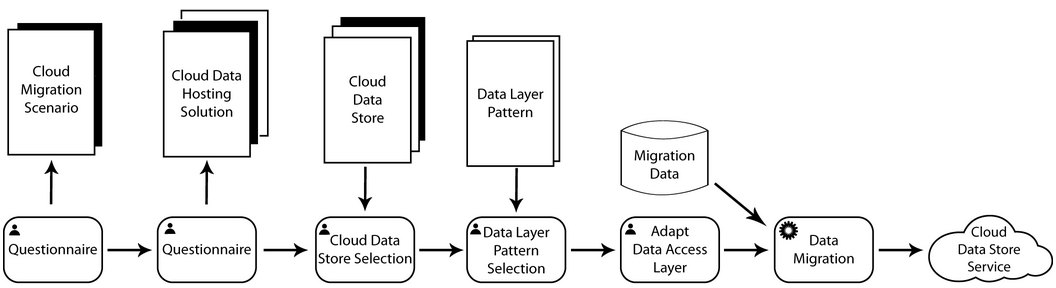
\includegraphics[clip, scale=0.4]{./gfx/clouddatamigrationtool.png}
	\caption[Cloud Data Migration Application - Cloud Data Migration Process]{Cloud Data Migration Process \cite{bachmann2012}} 
	\label{fig:cloudmigrateapp}
\end{figure}

In the \term{data layer pattern selection} and \term{adapt data access layer steps}, the user must specify how to connect to the data store his data is migrated to, and provide the necessary information to establish the connection. The extension of ServiceMix-mt for enabling Cloud data access support allows the user to select this prototype for transparently access the migrated data. 

\FloatBarrier
\section{Apache JMeter}
\label{sec:jmeter}  

Apache JMeter is a Java-based application which provides support for load testing and performance measurement \cite{jmeter2013}. It provides support for different communication protocols, e.g. \ac{HTTP}, \ac{SOAP}, database via \ac{JDBC}, etc. A multi-protocol support enables the application to be used for testing different layers of an application, e.g. presentation layer, and database layer. Furthermore, the user can configure in JMeter different load parameters, e.g. number of threads, iterations, etc., in order to build a heavy load simulation to run on the backend server. Simulation results are presented in structured formats for posterior analysis. 

In this diploma thesis we provide an evaluation of the behavior of the final prototype. Due to the \ac{JDBC} functionality supported by JMeter, we use it to generate the load test cases which are run on ServiceMix-mt.

\FloatBarrier
